\chapter{Progettazione}\label{chapter:progettazione}
%ecco qualche  commento.
%la sezione 4 richiede un po' di lavoro.
%manca tutto il livello di spiegazione tra l'introduzione e la sezione 4 attuale.
%in pratica devi raccontare in modo sintetico le strategie scelte (senza troppi dettagli
%implementativi), come hai organizzato le strutture di supporto
%e il perche'.
%Poi puoi raccontare lo pseudo codice, ma non nello stato attuale (riorganizzalo, semplificalo).
%Ci sta anche qualche disegno astratto sulla strategia di local search (puoi fare una griglia 2d
%che mostra il vicinato di traslazione o cose simili) ---> ?

%%% Sezione in cui spiegavo l'uso del biopython, causato dai file in ingresso che sono dei pdb
%%% Sezione sulle tecniche utilizate e le strutture dati che mi hanno aiutato all'interno del programma
%%% Poi avendo un approccio top-down spiego lo speudo codice
In questo capitolo viene affrontata la parte di implementazione e progettazione, vedremo le strategie di ricerca scelte, l'organizzazione delle strutture dati a supporto dell'esecuzione e poi avremo un approccio top-down verso il codice scritto. Introduco anche la libreria di supporto che ci ha permesso di svolgere il lavoro sul python.

\section{Librerie a supporto}\label{sec:libreriesupporto}  
In questo framework mi sono avvalso della libreria opensource \cite{BioPythonManual}. É una libreria di strumenti per la biologia computazionale e la bioinformatica. Essa contiene classi per rappresentare sequenze biologiche e annotazioni di sequenze ed è in grado di leggere e scrivere file provenienti da diversi formati. 
Questa libreria mi ha permesso di utilizzare il parser per i file pdb (Protein Data Bank) al cui interno sono codificate le informazioni riguardanti gli atomi come nome dell'atomo posizione all'interno dello spazio tridimensionale ed altre informazioni. Oltre a fornirmi un parser, al suo interno sono presenti dei moduli che permettono di generare oggetti come le catene, i residui e gli atomi stessi.
Questo da la possibilità di chiamare metodi specifici che semplificano il lavoro di gestione delle entità atomo, catena e residui. Viene fornita anche la possibilità di scrivere file in output nel formato desiderato (pdb), il che ci porta al secondo strumento utile il PyMOL. 

Il PyMOL è un opensuorce software di grafica 3D, che viene utilizzato per la rappresentazione di biomolecole. Come si può dedurre dalla parte iniziale del nomem si riferisce al linguaggio python. Risulta molto utile nella fase di verifica, ovvero quando si deve controllare ciò che è stato compiuto su una molecola. Fornisce un linguaggio di programmazione molto simile al python che permette di creare script per maneggiare e visionare le modifiche effettuate.
 
\section{Strategie di ricerca}\label{sec:Strategiediricerca}
All'interno di questo framework si è reso necessario utilizzare tecniche di ricerca locale nella fase in cui si cerca di andare a ristabilire il collegamento dei due loop alla parte mobile una volta effettuata una rotazione/traslazione su di essa. In questo caso la tecnica utilizzata è la hill-climbing, in cui si cerca di trovare il massimo (o il minimo) di una funzione di costo attraverso la ricerca di soluzioni vicine a quella corrente. In questo caso specifico, la funzione di ricerca cerca di ottimizzare la conformazione di un loop di collegamento alla volta attraverso la rotazione degli angoli torsionali. Si parte da una configurazione iniziale del loop rappresentata mediante ad una lista di residui, e cerco di migliorarla ruotando uno dei due angoli torsionali a disposizione, partendo da un residuo specificato. L'angolo torsionale viene scelto casualmente tra $\phi$ o $\psi$. Una volta applicata la rotazione viene restituita la nuova conformazione della proteina e si procede in questo modo fin tanto che non viene raggiunto il risultato desiderato. 

Viene utilizzata anche una tecnica di ricerca per guidare il processo che porta al completamento del percorso più breve tra le due configurazioni. La strategia di ricerca, in questo caso, è una forma di shortest path con una coda di priorità implementata tramite heap, albero binario ordinato. Essa viene utilizzata per selezionare il nodo con il costo totale (cioè il costo del percorso finora più la stima del costo rimanente) più basso in ogni iterazione. In questo modo si cerca di espandere i nodi che hanno costo totale più basso per primi. Ad ogni iterazione viene preso il vicinato del punto analizzato, si trasla in questi nuovi punti, come si può vedere in Fig. \ref{fig:Transizioni}. Per ogni transizione mediante un sistema di indici si risale ad un insieme di possibili rotazioni amiche, concetto che approfondiremo nelle sezioni successive, e dopodiché si prova la convergenza.

\begin{figure}[H]
	\centering
	\subfloat[][\emph{6 vicini}]
	{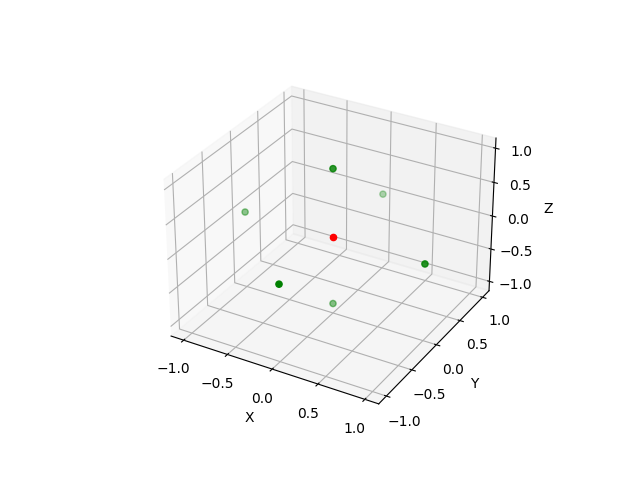
\includegraphics[width=0.5\textwidth]{Immagini/Transizioni_semplici.png}} 
	\subfloat[][\emph{26 vicini}]
	{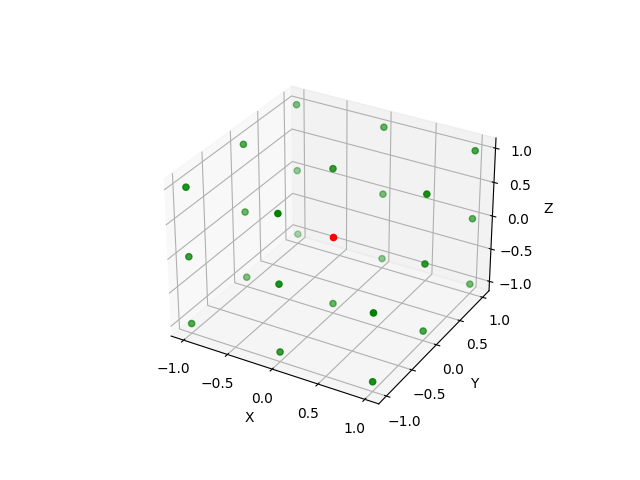
\includegraphics[width=0.5\textwidth]{Immagini/Transizioni_complesse.png}}
	\caption{In (\textbf{a}) vengono mostrati i 6 vicini come intorno del punto (0,0,0) contrassegnato di rosso; mentre in (\textbf{b}) vengono mostrati i 26 vicini di (0,0,0) contrassegnato sempre in rosso.}
	\label{fig:Transizioni}
\end{figure}

\section{Strutture dati a supporto}\label{sec:Strutturedati}
Le strutture dati sono importanti all'interno di un algoritmo, non solo per permettere di conservare informazioni, ma incidono anche sul tempo di esecuzione del singolo programma. Organizzare quindi l'accesso alle strutture dati nel modo migliore permette di risparmiare tempo d'esecuzione oltre a semplificare nella maggior parte dei casi la comprensione della stessa. 

Il linguaggio di programmazione scelto, python, necessità di studiare nel modo corretto come accedere alle strutture dati per evitare di trovarsi con dati inconsistenti poiché sono frutto di più modifiche. Per questo motivo e per quanto detto in precedenza io ho previsto 8 strutture di dati importanti: due dedicate a contenere la parte mobile e i loop, due dedicate al salvataggio delle posizioni acquisite da parte mobile e loop durante il cammino da una configurazione all'altra, due dedicate al salvataggio temporaneo e al ripristino in caso di clash delle coordinate dei loop pre e post rotazione, due dedicate alla gestione dei clash e due dedicate al concetto di amicizia delle matrici di rotazione pre-calcolate.

Le strutture dati sono state quasi tutte sviluppate come dei dizionari ad accesso chiave valore. Per quanto riguarda la struttura dati dedicata al controllo della presenza dei clash, la struttura contiene tuple di coordinate tridimensionali e per ciascuna tupla è contenuto la catena il residuo e l'atomo che si trovano in quella posizione. Questo è stato possibile mediante una discretizzazione di tutti gli atomi all'interno di una matrice tridimensionale. Chiaramente il passo di campionamento può essere impostato mediante costante, di default è impostato a 5 Ångström. \footnote{Ångström, sono un'unità di misura, non SI, pari a $10^-10m$.} 

Per quanto riguarda le strutture dati per mantenere salvate le coordinate dei loop e della parte mobile anch'esse sono organizzate come dizionari la cui chiave indicizza l'insieme delle varie coordinate. Le chiavi che indicizzano la struttura sono degli interi calcolati nel seguente modo:
$$
	key = x + y \cdot dx + z \cdot dx \cdot dy + r \cdot dx \cdot dy \cdot dz
$$
In questo caso $x, y, z$ identificano la traslazione che abbiamo effettuato sulla parte mobile, $r$ identifica univocamente la rotazione applicata alla parte mobile, mentre $dx, dy, dz$ sono le grandezze che su ogni asse separano la configurazione aperta da quella chiusa. Attraverso metodi di get e set possiamo settarli nelle variabili coinvolte nel processo evitando problemi di condivisione della memoria.

Abbiamo due dizionari dedicati al salvataggio temporaneo e al ripristino delle coordinate nel caso la rotazione non sia buona. Questi dizionari sono solamente per i due loop all'interno della funzione che si occupa di farli convergere alla parte mobile. La struttura dedicata ai loop e alla parte mobile invece sono due liste che a loro volta contengono residui a cui applicare le varie rotazioni. 

Le ultime due strutture dati nominate, utilizzate per il concetto di amicizia, sono a loro volta dei dizionari indicizzati per chiave, dove la chiave è appunto l'indice $r$ nominato in precedenza che identifica univocamente all'interno di queste strutture una matrice di rotazione e i suoi amici visti come una lista di indici.

Voglio comunque porre enfasi sullo studio necessario per progettare la singola struttura che mi ha concesso non solo di risolvere il problema della condivisione della memoria, ma anche di velocizzare il processo di accesso alla struttura dati e quindi portare più velocità nell'esecuzione della ricerca locale.

\section{Approccio Top-Down al codice}\label{sec:ApproccioTopDown}
Analizziamo lo pseudo-codice che permette di compiere il lavoro preposto dall'obbiettivo. 

\begin{algorithm}
	\caption{Inizializzazione framework}
	\label{alg:inizializzazione}
	\begin{algorithmic}
		\State $parser \gets PDBParser(PERMISSIVE=True, QUIET=True)$
		\State $covidchiusa \gets parser.getstructure(titleclosed)$
		\State $covidaperta \gets parser.getstructure(titleopen)$
		\State $calcoloamici(DIV)$
		\State $ptmob \gets partemobile(listacatene, catenainteresse)$
		\State $centroide \gets calcolocentroide(ptmob)$
		\State $normalizzazionestruttura(covidchiusa, covidaperta, centroide)$
		\State $calcoloparallelepipedo(covidchiusa, covidaperta)$
		\State $loop \gets identifyloop(listacatene, catenainteresse, costantiA)$
		\State $coil \gets [loop]$
		\State $loop \gets identifyloop(listacatene, catenainteresse, costantiB)$
		\State $loopr \gets loop[::-1]$
		\State $coil.append(loopr)$
		\State $salviamo(coildictcoordinates)$
		\State $key = x + y \cdot dx + z \cdot dx \cdot dy + r \cdot dx \cdot dy \cdot dz$
		\State $ptmob \gets partemobile(listacatene, catenainteresse)$
		\State $storedptmob \gets salviamo(ptmob)$
		\If{$key \notin posizioniacquisiteptmob$}
		\State $insert(posizioniacquisite, key)$
		\EndIf
		\State $residuipartefissa \gets partefissa(listacatene, catenainteresse)$
		\State $coordinate \gets salviamo(coildictcoordinates)$
		\If{$key \notin posizioniacquisiteloop$}
		\State $insert(posizioniacquisiteloop, key)$
		\EndIf
		\State $nuova\_chiave, prev \gets shortest\_path(key)$
		\State $printpdb(configurazioni)$
	\end{algorithmic}
\end{algorithm}

Come si può vedere in \ref{alg:inizializzazione} si vanno ad inizializzare le componenti principali del sistema. Innanzitutto viene creato un parser che ha il compito di parsare il file pdb in ingresso. Mediante il parser vengono estratte le configurazioni dai file pdb. Dopodiché vengono calcolate le matrici di rotazione e il concetto di amicizia tra matrici di rotazione, come riportato in \ref{subsec:amiciziarotazioni}. Una volta fatto, calcoliamo il centroide della parte mobile aperta e normalizziamo la struttura chiusa e aperta, in modo da averle centrate in (0,0,0). Dopodiché si restringe lo spazio di ricerca, come mostrato in \ref{subsec:areadiricerca}.

Una volta terminata la fase di inizializzazione, vengono presi i loop normalizzati, la parte mobile della configurazione chiusa normalizzata e la parte fissa utile per la gestione dei clash. Generiamo la chiave che ci permette di salvare le informazioni e cominciamo a cercare convergenza tra le due configurazioni mediante \ref{sec:shortestpath}.

\subsection{Amicizia tra matrici di rotazione}\label{subsec:amiciziarotazioni}

Utilizzando il metodo descritto in \ref{subsec:superfibonaccispiral}, si possono generare un insieme di vettori $x$ che rappresentano i vettori $x$ delle matrici di rotazione tridimensionale che verranno poi utilizzate per ruotare la parte mobile. 

Il concetto di amicizia tra due matrici è relativo al prodotto scalare tra i vettori $x$ e $y$ di due matrici. In questo caso è necessario definire delle soglie per discriminare una matrice piuttosto che un altra, le soglie impostate sono per quanto riguarda il prodotto scalare dei vettori $x$ $0.94$, mentre per i vettori $y$ $0.87$. Vengono impostate queste soglie poiché nel nostro caso il prodotto scalare dei vettori è compreso tra $[-1, +1]$, dove $+1$ rappresenta l'ugualianza dei due vettori, mentre $-1$ rappresenta la completa estraneità dei due vettori. 
Vengono scelte le seguenti soglie, perché vogliamo rendere piccolo lo spostamento da una matrice all'altra quando vengono applicate alla parte mobile; infatti, movimenti più piccoli garantiscono una migliore probabilità di convergenza tra i loop e la parte mobile. 

L'algoritmo proposto \ref{alg:calcoloamici} permette di ottenere il risultato mostrato in Fig. \ref{fig:Tagliox}, il parametro scelto è 20, che permette di generare 400 diversi vettori $x$ che a loro volta danno vita a 8000 matrici, in questo modo attraverso le soglie impostate in precedenza possiamo ottenere circa 3 o 4 migliaia di matrici amiche. 

\begin{figure}[H]
	\centering
	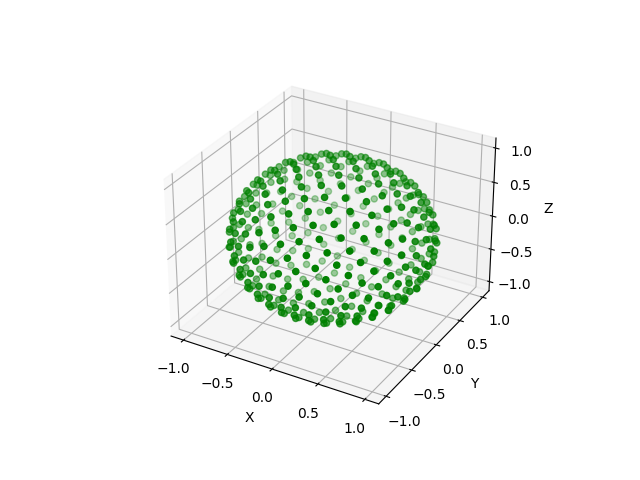
\includegraphics[width=0.6\textwidth]{Immagini/Tagliox.png}
	\caption{Punti equidistanti sulla superficie di una sfera, creando una distribuzione uniforme degli stessi.}
	\label{fig:Tagliox}
\end{figure}

\begin{algorithm}
	\caption{Procedura che permette il calcolo degli amici.}
	\label{alg:calcoloamici}
	\begin{algorithmic}
		\Procedure{calcoloamici}{$DIV$}
		\State $sphere \gets []$
		\State $n1 \gets DIV$
		\State $n \gets n1 * n1$
		\State $golden\_angle \gets 3.1415 \cdot (3 - \sqrt{5})$
		\For{$i$ \textbf{in} $range(n)$}
		\State $\theta \gets golden\_angle \cdot i$
		\State $pos \gets float(i / (n-1))$
		\State $z \gets (1-1.0/n-(1.0/n-1))\cdot pos+(1.0/n-1)$
		\State $radius \gets \sqrt{1 - z \cdot z}$
		\State $temp \gets [0, 0, 0]$
		\State $temp[2] \gets radius \cdot \cos(\theta)$
		\State $temp[1] \gets radius \cdot \sin(\theta)$
		\State $temp[0] \gets -z$
		\State $sphere.append(temp)$
		\EndFor
		\For{$x, j$ \textbf{in} $zip(sphere, range(len(sphere)))$}
		\State $multiplier \gets [0, 0, 1]$
		\If{$j == 0$}
		\State $multiplier \gets [0, 0, -1]$
		\EndIf
		\State $y \gets \langle x,multiplier \rangle$
		\State $y\_norm \gets normalizza(y)$
		\State $z \gets \langle x,y \rangle$
		\State $z\_norm \gets normalizza(z)$
		\For{$i$ \textbf{in} $range(DIV)$}
		\State $angle \gets radians((360/DIV*i))$
		\State $y_new \gets y_norm\cdot\cos(angle) - z\cdot\sin(angle)$
		\State $z_new \gets y_norm\cdot\sin(angle) + z\cdot\cos(angle)$
		\EndFor
		\EndFor
		\State $amici \gets amici(0.94, 0.87)$ 
		\EndProcedure
	\end{algorithmic}
\end{algorithm}

\subsection{Riduzione area di ricerca}\label{subsec:areadiricerca}
Restringere l'area di ricerca è fondamentale per non perdere tempo computazionale in zone dello spazio tridimensionale che non sono utili ai fini della ricerca. Per questo ho sviluppato la seguente funzione \ref{alg:parallelepipedo}.
\begin{algorithm}
	\caption{Calcolo del parallelepipedo}
	\label{alg:parallelepipedo}
	\begin{algorithmic}
		\Procedure{calcoloparallelepipedo}{$chiusa, aperta$}
		\State $mobilclosedpart \gets partemobile(listacatene, catenainteresse)$
		\State $mobilopenedpart \gets partemobile(listacatene, catenainteresse)$
		\State $ca \gets$ \Call{calcolocentoide}{$mobilopenedpart$}
		\State $cc \gets$ \Call{calcolocentoide}{$mobilclosedpart$}
		\State $x\_parallelepipedo\_min \gets$ \textit{int}$(min(0,(ca[0]-cc[0])-1))$
		\State $x\_parallelepipedo\_max \gets$ \textit{int}$(max(0,(ca[0]-cc[0])+1))$
		\State $y\_parallelepipedo\_min \gets$ \textit{int}$(min(0,(ca[1]-cc[1])-1))$
		\State $y\_parallelepipedo\_max \gets$ \textit{int}$(max(0,(ca[1]-cc[1])+1))$
	    \State $z\_parallelepipedo\_min \gets$ \textit{int}$(min(0,(ca[2]-cc[2])-1))$
		\State $z\_parallelepipedo\_max \gets$ \textit{int}$(max(0,(ca[2]-cc[2])+1))$
		\State $dx \gets x\_parallelepipedo\_min - x\_parallelepipedo\_max$
		\State $dy \gets y\_parallelepipedo\_min - y\_parallelepipedo\_max$
		\State $dz \gets z\_parallelepipedo\_min - z\_parallelepipedo\_max$
		\EndProcedure
	\end{algorithmic}
\end{algorithm}
In questo modo riusciamo a restringere il campo di lavoro, ad una sorta di parallelepipedo che contiene entrambe le configurazioni. Il parallelepipedo è individuato dalle coordinate per ogni asse massime e minime e dopodiché possiamo verificare l'appartenenza all'interno dello stesso mediante una semplice funzione che verifica l'appartenza. All'interno di questa funzione vengono anche calcolati gli indici che permettono di calcolare la chiave di indicizzazione di ogni nodo generato.  

\section{Shortest-Path}\label{sec:shortestpath}
Come descritto in \ref{chapter:obbiettivi}, l'obbiettivo è quello di convergere tra la conformazione chiusa e quella aperta mediante il cammino con il minor costo possibile.
Per fare ciò lavoriamo e ci concentriamo esclusivamente sulla conformazione chiusa, l'utilizzo della conformazione aperta è esclusivamente necessario per verificare il raggiungimento dell'obiettivo. 

Terminando la fase di inizializzazione in \ref{alg:inizializzazione}, si procede nel individuare e salvare i loop, che mettono in collegamento la parte mobile con la parte fissa. I due loop sono simili, ma diversi nella direzione da loro presa, ovvero il loop-A si dirige dalla parte fissa alla parte mobile, mentre il loop-B lavora al contrario quindi per rendere omogeneo il comportamento del programma nei confronti dei due loop è necessario capovolgere il secondo. Questo non comporta nessun altra modifica, è però necessario ricordarsi di capovolgere il loop nel momento in cui si effettua il processo di scrittura file. Le costanti sul posizionamento dei loop sono state fornite insieme alle configurazioni ed è importante sottolineare che è stato preso un residuo in più in capo e in coda al loop, per verificare che ogni modifica si adatti bene alla struttura a cui si deve attaccare. Una volta che abbiamo terminato l'attività di salvataggio dei loop e della parte mobile avviamo shortest-path \ref{alg:algoritmoshortpath} e una volta concluso stampiamo passo passo le configurazioni intermedie. 

\begin{algorithm}
	\caption{Shortest-Path}
	\label{alg:algoritmoshortpath}
	\begin{algorithmic}
		\Procedure{Shortest-path}{$start\_idx$}
		\State $heap \gets [(0, start\_idx)]$
		\State $prev \gets \{\}$, $costo \gets \{\}$
		\State $prev[start\_idx] \gets -1$, $costo[start\_idx] \gets 0$
		\While {heap}
		\State $cost, indice\_current \gets heap$
		\State $movimento, r \gets indice\_current$
		\State $ptmob \gets load(indice\_current)$, $loop \gets load(indice\_current)$
		\State $friends \gets amici(r)$
		\For {$traslazione$ \textbf{in} $traslazioni$}
		\For {$r2$ \textbf{in} $friend$}
		\State $ptmob \gets load(r2)$, $ptmob \gets applytransition(traslazione)$
		\If {\textbf{not} $is\_allowed(ptmob)$}
		\State \textbf{continue}
		\EndIf
		\State $pre-processing(ptmob)$
		\State $convergenza \gets esecuzione\_rotazioni()$
		\If {$convergenza$}
		\State $nuovo\_indice \gets indice\_current$
		\State $nuovo\_costo \gets costo + costo(r, r2)$
		\If {$nuovo\_costo < costo[indice\_current]$}
		\State $prev[nuovo\_indice] \gets indice\_current$, 
		\State $costo[nuovo\_indice] \gets nuovo\_costo$
		\State $heap \gets (nuovo\_indice, nuovo\_costo)$
		\State $insert(posizioniacquisiteloop, nuovo\_indice)$
		\State $insert(posizioniacquisiteloop, nuovo\_indice)$
		\If {$dist(ptmob, covid\_aperta) < 0.1$}
		\State \textbf{return} $nuovo\_indice, prev$
		\EndIf
		\EndIf
		\EndIf 
		\EndFor
		\EndFor
		\EndWhile 
		\EndProcedure
	\end{algorithmic}
\end{algorithm}
Come descritto in \ref{alg:algoritmoshortpath}, viene utilizzata una coda di priorità implementata tramite heap, albero binario ordinato, in cui passo passo vengono inseriti i nuovi nodi scoperti. Si inizia iterando sulla struttura dati, e si estrae il nodo che ha costo minore. Una volta estratto il nodo, prendiamo l'indice e ne ricaviamo la traslazione che fino a quel momento ci ha permesso di arrivare in quella posizione e la rotazione della parte mobile. Recuperiamo e settiamo nuovamente le coordinate alla parte mobile e ai loop, in modo tale da ripartire da dove eravamo rimasti. Una volta estratte le rotazioni amiche dell'attuale, si cercano nuove soluzioni. 

Per ogni traslazione elencate nell'array traslazioni, come in Fig. \ref{fig:Transizioni}, e per ogni rotazione amica si cerca convergenza. Prima di raggiungere se possibile la convergenza è necessario effettuare delle operazioni, ovvero dobbiamo caricare la parte mobile nella determinata rotazione $r2$ poiché tutte le rotazioni sono pre-calcolate in modo da ridurre il tempo di esecuzione; dobbiamo traslare la parte mobile nella corretta posizione fornita dagli indici. Una volta posizionata correttamente la parte mobile è necessario effettuare il controllo che la parte mobile sia all'interno del parallelepipedo, per i motivi descritti in \ref{subsec:areadiricerca}, dopodiché se la rotazione è consentita dobbiamo effettuare il pre-processing per determinare le strutture che permettono di comprendere la presenza di clash quando si ruotano i residui che compongono i loop. 

Terminata la fase di pre-processing necessaria all'individuazione di clash, si procede alla convergenza, ovvero si cerca di far convergere i loop alla nuova posizione della parte mobile, vedremo più nel dettaglio questa funzione nella prossima sottosezione. Se viene raggiunta convergenza, nella maggior parte dei casi è cosi perché gli spostamenti sono relativamente piccoli a meno di clash insormontabili, va inserito all'interno dell'heap il nuovo nodo se e soltanto se il nuovo costo è migliore del costo già presente per quel nuovo indice nel dizionario dei costi. Il nuovo costo viene calcolato come descritto in \ref{subsec:calcolocostoarco}. Se effettivamente minore inseriamo il nuovo costo ed è anche necessario aggiornare anche il nodo precedente che ci ha permesso di arrivare a questo nodo nella struttura prev. 

Se abbiamo raggiunto convergenza è necessario poi salvare le nuove coordinate sia dei loop che della parte mobile. É importante anche capire se abbiamo ottenuto il nostro obbiettivo principale ovvero se siamo arrivati a convergenza tra le due configurazioni, quella attuale e quella aperta, per fare ciò utilizziamo semplicemente la distanza euclidea tra la configurazione attuale e quella di arrivo. La soglia impostata per terminare il lavoro è 0.1 A che garantisce l'effettiva convergenza. 

\subsection{Calcolo costo arco}\label{subsec:calcolocostoarco}
La parte più importante all'interno dell'algoritmo di shortest-path è quello di calcolare il costo del nodo che si sta analizzando. Il nostro costo viene calcolato mediante 3 contributi: il primo è il costo del movimento delle coordinate; il secondo è costo dell'amicizia tra le matrici di rotazione; il terzo è lo spostamento dall'asse centrale che supponiamo essere il percorso migliore.

Analizzando nel dettaglio le componenti troviamo che il costo del puro movimento è costante a 1, poiché che ci si muova in negativo o in positivo il delta di spostamento è 1 a patto che venga utilizzato il vicinato di transizione semplice (Fig. \ref{fig:Transizioni} \textbf{a}). 

Il costo dell'amicizia tra due matrici è estratto come prodotto scalare dei due vettori $x$ e $y$, però preso in questo modo, ovvero $(1-\langle x, x2\rangle) + (1-\langle y, y2\rangle)$. In questo il costo di amicizia ci permette di pagare poco se ci muoviamo poco, mentre pagare un costo elevato se decidiamo di effettuare un movimento elevato. 

Il terzo componente è dedicato alla distanza del nuovo centroide generato dal segmento, ovvero se ci allontaniamo dall'ipotetico percorso migliore paghiamo una penalità. Questo coefficente viene calcolato come la distanza tra un punto e un segmento usando la proiezione ortogonale del punto sul segmento e la distanza euclidea tra il punto originale e il punto proiettato sul segmento.

Queste tre componenti determinano il costo del nuovo nodo generato, privilegiando i nodi più vicini al percorso ottimale e lasciando lo sviluppo dei nodi pù marginali in fondo.

\subsection{Convergenza tra loop e parte mobile}\label{subsec:convergenza}
\begin{algorithm}
	\caption{Esecuzione rotazioni tra loop e parte mobile}
	\label{alg:algconvergenza}
	\begin{algorithmic}
		\Procedure{esecuzione\_rotazioni}{ptmob}
		\State $distanza\_iniziale \gets [0,0]$
			\For{$loop$ \textbf{in} $coil$}
		\State $distanza\_iniziale[idx] \gets$ \Call{objective\_function}{$loop$, $ptmob$}
		\EndFor
		\State $angle\_to\_direction \gets$ \Call{suggestedsetofangle}{180, 1}
		\For{$a$ \textbf{in} $angle\_to\_direction$}
			\For{$loop$ \textbf{in} $coil$}
				\If{($distanza\_iniziale[idx] \geq 0.1000$)}
					\State $res \gets$ \textit{int}(\textit{len}($loop$)) $-$ 2
					\State $prova \gets$ \Call{hillclimbing}{$loop$, $residui\_costanti[idx]$, $a$, $res$}
					\State $distance \gets$ \Call{objective\_function}{$prova$, $ptmob$}
					\If{($distance < distanza\_iniziale[idx]$)}
						\State $clash \gets$ \Call{searchneighbor}{$prova$}
						\If {\textbf{not} ($clash$)}
							\State $distanza\_iniziale[idx] \gets distance$
							\State $storage(prova, idx)$
						\EndIf
					\EndIf
				\EndIf
				\State $load(loop, idx)$
			\EndFor
		\EndFor
		\For {$i$ \textbf{in} \textit{range}(iterazioni\_massime)}
		\For{$loop$ \textbf{in} $coil$}
		\If {\textbf{not} stop\_loop[idx]}
		\State $stop\_loop[idx] \gets$ \Call{stopsearch}{}
		\If{($distanza\_iniziale[idx] \geq 0.1000$)}
		\State $n\_res \gets$ \Call{suggestedresidue}{\textbf{len}(loop)}
		\State $angle \gets$ \Call{suggestedangle}{distanza\_iniziale[idx]}
		\State $swap \gets$ \Call{suggestedchange}{distanza\_iniziale[idx]}
		\State $loop\_new \gets$ \Call{hillclimbing}{$loop$, $residui\_costanti[idx]$, $angle$, $n\_res$}
		\State $distance \gets$ \Call{objective\_function}{$loop\_new$, $ptmob$}
		\If{($distance < distanza\_iniziale[idx]$)}
		\State $clash \gets$ \Call{searchneighbor}{$prova$}
		\If {\textbf{not} ($clash$)}
		\State $distanza\_iniziale[idx] \gets distance$
		\State $storage(prova, idx)$
		\EndIf
		\EndIf
		\State $load(loop, idx)$
		\EndIf
		\EndIf
		\EndFor
		\EndFor
		\If {$distanza\_iniziale[0] \leq 0.1$ \textbf{and} $distanza\_iniziale[1] \leq 0.1$}
		\State \textbf{return} \textit{True}
		\EndIf
		\State \textbf{return} \textit{False}
		\EndProcedure
	\end{algorithmic}
\end{algorithm}

La parte più importante è appunto questa che si occupa della convergenza dei loop, verso la nuova conformazione della parte mobile. Innanzitutto viene calcolata la distanza che i loop devono colmare fra se stessi e i punti di aggancio della parte mobile, che avviene mediante la funzione $objective\_function$(\ref{subsubsec:funzionetarget}). 

Una volta misurata la distanza da colmare, effettuando vari test, ho riscontrato che è possibile dare una mano alla convergenza dei loop, praticando delle rotazioni preliminari su un ampio spettro di angoli da $\ang{-180}$ a $\ang{180}$ con passo di campionamento $1$. Ogni angolo viene provato per ciascun angolo torsionale. Per effettuare la singola rotazione utilizziamo la funzione $hillclimbing$(\ref{subsubsec:hillclimbing}). Una volta effettuata la singola rotazione e propagata all'interno del loop è necessario, se la distanza risultante è minore della precedente si procede a verificare la presenza di clash per garantire la stabilità della proteina. 

Tutto ciò avviene grazie alla funzione $searchneighbor$(\ref{subsubsec:ricercavicini}), che si avvale di ciò che è stato fatto durante il pre-processing descritto in precedenza. Se non vengono riscontrati clash, la rotazione viene considerata valida e vengono aggiornate le coordinate nelle strutture dati a supporto dell'esecuzione.

Una volta terminata la fase di applicazione di queste rotazioni canoniche, si passa alle iterazioni che lavorano di fino in base alla distanza del loop. Come prima cosa ci si chiede se questo loop è stato fermato nella sua progressione perché, se è cosi non ha senso continuare a iterare se almeno uno dei loop non può raggiungere la meta. Se il loop non è ancora stato fermato verifichiamo che al giro successivo non debba essere fermato mediante la funzione $stopsearch$. Questa funzione agisce sulle distanze raggiunte nel corso delle iterazioni dal loop e calcola un indice di incremento tra le ultime 20 distanze raggiunte. Questo indice è sicuramente negativo perché la distanza decresce, se però è maggiore di $-0.01$ significa che la distanza raggiunta nel corso delle 20 distanze ha una differenza che è troppo piccola per proseguire il lavoro. Ovviamente ho eseguito vari test per trovare la soglia e il numero di distanze da prendere in considerazione ed ho cercato il miglior compromesso per evitare di fermare troppo presto il cammino del loop. 

Se il loop non è stato fermato allora devono essere determinati alcuni parametri: il residuo su cui lavorare, che viene determinato in modo casuale; l'angolo con cui provare la successiva rotazione determinato dalla funzione $suggestedangle$(\ref{subsubsec:suggerimentoangoli}); lo swap che interviene per cercare di smuovere il processo di convergenza del loop nel caso si raggiunga un "asintoto". Nel caso in cui venga richiesto uno swap, si effettuano delle rotazioni di $\ang{-0.5}$ e $\ang{0.5}$ sulla base del loop per smuovere il processo. Una volta effettuata la singola rotazione e propagata all'interno del loop è necessario, se la distanza risultante è minore della precedente, verificare la presenza di clash per garantire la stabilità della proteina.

Le iterazioni possono terminare per i seguenti motivi:
\vspace{10pt}
\begin{itemize}
	\item entrambi i loop raggiungono la distanza minima quindi la funzione restituisce l'avvenuta convergenza;
	\vspace{5pt}
	\item uno dei loop è stato fermato durante il processo di convergenza, quindi la funzione restituisce che la convergenza non è avvenuta;
	\vspace{5pt}
	\item uno dei due loop non ha colmato la distanza, quindi la convergenza non è avvenuta.
\end{itemize}

\subsubsection{Funzione obbiettivo}\label{subsubsec:funzionetarget}
La funzione obiettivo, \ref{alg:funzioneobj}, viene utilizzata per calcolare la distanza tra l'ultimo residuo del loop e la parte di attacco della parte mobile corrispondente. La distanza viene misurata mediante due contributi: il primo deriva dalla distanza euclidea dei due atomi carbonio $\alpha$; il secondo contributo è dato dal prodotto scalare dei due vettori tra gli atomi carbonio e azoto dell'ultimo residuo della parte mobile e del loop. 

É necessario considerare il prodotto scalare tra i due vettori, poiché è necessario che i due residui interagiscano nel modo corretto; infatti, i due atomi carbonio $\alpha$ potrebbero essere a contatto, ma i due atomi di carbonio e azoto potrebbero essere opposti e non favorire il legame tra i due residui. 
 
\begin{algorithm}
	\caption{Objective Function}
	\label{alg:funzioneobj}
	\begin{algorithmic}
		\Function{objective\_function}{$loop, ptmob$}
		\State $residuo\_loop \gets loop[resiude]$
		\State $residuo\_ptmob \gets ptmob[residue]$
		\State $distanzaCA \gets residuo\_loop[CA] - residuo\_ptmob[CA]$
		\State $asse\_loop \gets residuo\_loop[N] - residuo\_loop[C]$
		\State $asse\_loop \gets normalizza(asse\_loop)$
		\State $asse\_ptmob \gets residuo\_ptmob[N] - residuo\_ptmob[C]$
		\State $asse\_ptmob \gets normalizza(asse\_ptmob)$
		\State $prodotto\_scalare \gets \langle asse\_loop, asse\_ptmob \rangle$
		\State $product \gets (\sqrt{1-prodotto\_scalare}/2)$
		\State \textbf{return} $distanzaCA \cdot (1 + product)$
		\EndFunction
	\end{algorithmic}
\end{algorithm}

\subsubsection{Hillclimbing}\label{subsubsec:hillclimbing}
La funzione $hillclimbing$, \ref{alg:hillclimbing}, viene utilizzata per applicare il movimento ad un residuo e poi propagarlo al resto del loop. A seconda dell'angolo torsionale estratto necessitiamo di generare una matrice di rotazione differente. Nel caso $0$, ovvero $\phi$, costruiamo la matrice di rotazione sull'asse degli atomi C$\alpha$-N; nel caso $1$, ovvero $\psi$, costruiamo la matrice di rotazione sull'asse degli atomi C$\alpha$-C. Una volta calcolata la matrice la applichiamo ai residui a partire da quello scelto in modo randomico in precedenza. E' necessario controllare nel caso del loop-A di non applicare la rotazione in alcuni particolari residui che fanno parte del $\beta$-foglietto rigido. 
\begin{algorithm}[H]
	\caption{Hillclimbing}
	\label{alg:hillclimbing}
	\begin{algorithmic}
		\Function{hillclimbing}{$loop, angolo, idx\_rex$}
		\State $torsional\_angle \gets random(0,1)$
		\State $loop\_new \gets []$
		\If {$torsional\_angle == 0$}
		\State $asse \gets loop[idx\_rex][CA] - loop[idx\_rex][N]$
		\State $asse \gets normalizza(asse)$ 
		\State $rotation\_matrix \gets matrice(asse, angolo)$
		\Else
		\State $asse \gets loop[idx\_rex][CA] - loop[idx\_rex][C]$
		\State $asse \gets normalizza(asse)$ 
		\State $rotation\_matrix \gets matrice(asse, angolo)$
		\EndIf
		\For {$i$ \textbf{in} \textit{range}(0, idx\_rex)}
		\State $loop\_new \gets loop[i]$
		\EndFor
		\For {$i$ \textbf{in} \textit{range}(idx\_rex, \textit{len}(loop))}
		\State $loop\_new \gets ruota(loop[i])$
		\EndFor 
		\State \textbf{return} $loop\_new$
		\EndFunction
	\end{algorithmic}
\end{algorithm}
\subsubsection{SearchNeighbor}\label{subsubsec:ricercavicini}
La funzione $searchneighbor$, \ref{alg:searchnei}, si occupa di verificare la presenza di clash, ovvero interazioni tra atomi come descritto in \ref{subsec:ramachandranPrinciple}. In questo caso è necessario verificare sia che siano presenti clash tra i due loop, poiché sono a stretto contatto, e sia che siano presenti con gli altri atomi presenti nella proteina. L'unico modo per verificare la presenza di un clash è quella di controllare che la distanza euclidea tra due atomi sia maggiore rispetto alla somma dei rispettivi raggi di van der Walls.  
\begin{algorithm}[H]
	\caption{Searchneighbor}
	\label{alg:searchnei}
	\begin{algorithmic}[1]
		\Procedure{searchneighbor}{$residuo$}
		\State $res_linked \gets []$
		\If{$residue.id[1] \in side_chain_processed[idx_loop]$}
			\State $res_linked \gets side_chain_processed[idx_loop][residue.id[1]]$
		\EndIf
		\For{atom \textbf{in} residue}
			\If{atom.id \textbf{in} res\_linked}
				\For{atom\_check \textbf{in} res\_linked[atom.id]}
					\State $d \gets (atom\_check - atom)$
					\State $r \gets raggio(atom\_check)+raggio(atom)$
					\If{d $<$ r}
						\State \textbf{return} \textbf{True}
					\EndIf
				\EndFor
			\EndIf
			\State coordinate $\gets$ atom.get\_coord()
			\State key $\gets$ $(mx, my, mz)$
			\State six\_coord $\gets$ catch\_coordinates(key)
			\For{coord \textbf{in} six\_coord}
				\For{element \textbf{in} tridimensional\_clash[coord]}
					\State chain $\gets$ element['chain']
					\State atom\_to\_analize $\gets$ element['atom']
					\If{\textbf{not} same(atom, chain, residue)}
						\State $d \gets (atom\_to\_analize - atom)$
						\State $r \gets (raggio(atom\_to\_analize)+raggio(atom)$
						\If{d $<$ r}
							\State \textbf{return} \textbf{True}
						\EndIf
					\EndIf
				\EndFor
			\EndFor
		\EndFor
		\State \textbf{return} \textbf{False}
		\EndProcedure
	\end{algorithmic}
\end{algorithm}
\subsubsection{Suggestedangle}\label{subsubsec:suggerimentoangoli}
La funzione $suggestedangle$, \ref{alg:suggestedangle}, mi permette di determinare un angolo a partire dalla distanza residua. Questa funzione mi permette di avere un angolo piccolo quando la distanza è molto piccola e un angolo abbastanza grande quando la distanza è elevata(Fig. \ref{fig:fundis}). 

\begin{figure}
	\centering
	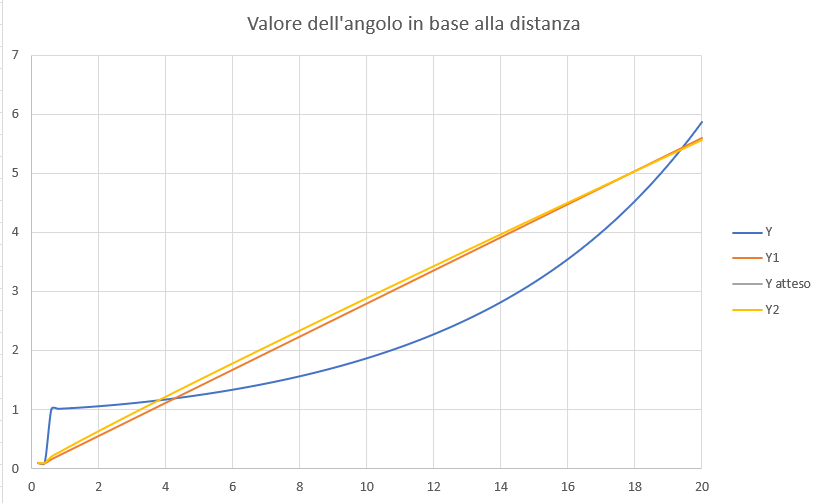
\includegraphics[width=0.6\textwidth]{Immagini/Funzionedistanza.png}
	\caption{La funzione Y2 è quella che mi permette di descrivere meglio il comportamento richiesto.}
	\label{fig:fundis}
\end{figure}

\begin{algorithm}
	\caption{SuggestedAngle}
	\label{alg:suggestedangle}
	\begin{algorithmic}
		\Function{suggestedangle}{$distanza$}
		\State $angle \gets 0.1$
		\If {$distanza \geq 0.5$}
		\State $angle \gets (2^{distanza^{-0.1}}\cdot distanza/6)$
		\EndIf
		\State \textbf{return} $angle$
		\EndFunction
	\end{algorithmic}
\end{algorithm}